\chapter{The ATLAS Experiment at the LHC}
\label{chap:atlas_experiment}
The ATLAS experiment is one of the four major experiments at the LHC at the European Organization for Nuclear Research (CERN). The ATLAS detector is designed as a general-purpose particle physics experiment, together with the CMS experiment. In Section~\ref{sec:atlas:lhc}, a brief description of the LHC is given, and in Section~\ref{sec:atlas:detector}, the ATLAS detector and its sub-detector systems are described.

\section{The Large Hadron Collider}
\label{sec:atlas:lhc}

The LHC is the world's largest synchrotron accelerator ($pp$ collider) located at CERN near Geneva, Switzerland. The LHC's circular beam pipes are 27 km in circumference, and two beams of protons are accelerated in opposite direction producing $pp$ collisions at $\sqrt{s} = $ 13 TeV in Run II. Separate magnet systems are used to direct proton beams in each direction.

\begin{figure}[!htb]
    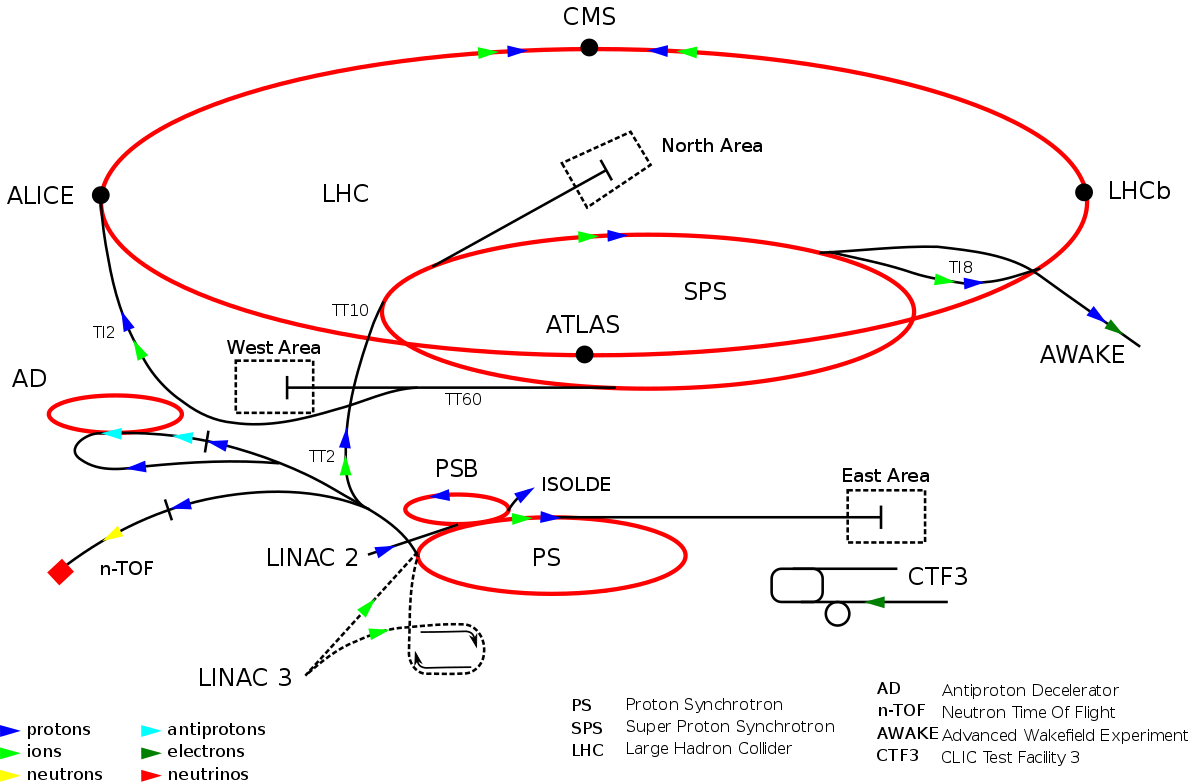
\includegraphics[width=0.8\textwidth]{figures/lhc.png}
    \centering
    \caption{LHC accelerator system and the four main experiments.}
    \label{fig:lhc}
\end{figure}

There are 8 interaction regions (IRs) at which two proton beams cross, and protons beams are injected into the LHC from two IRs. Before protons are injected to the LHC, they undergo a multi-stage acceleration by several accelerators~\cite{Bruning:782076}: a linear accelerator (LINAC2), the Proton Synchrotron Booster, the Proton Synchrotron (PS), and the Super Proton Synchrotron (SPS). The proton beams are accelerated up to 450 GeV when they are injected to the LHC with a 25 ns bunch spacing in Run II. There are more than $10^{11}$ protons in each bunch, and the large number of protons in each bunch results in multiple collisions per bunch crossing, knowns as \textit{pile-up}. In 2016, the mean number of interactions per bunch crossing was $\langle\mu\rangle = 24.9$.

The four main experiments at CERN are distributed around the LHC at collision points. Two experiments, ATLAS and CMS, are designed as general purpose experiments, and A Large Ion Collider Experiment (ALICE) and the Large Hadron Collider beauty (LHCb) are designed to study strong interaction using heavy ion collisions and the matter-antimatter asymmetry using b quarks, respectively. Figure~\ref{fig:lhc} shows the four main experiments and the accelerators at the LHC.


\section{The ATLAS detector}
\label{sec:atlas:detector}

\begin{figure}[!htb]
    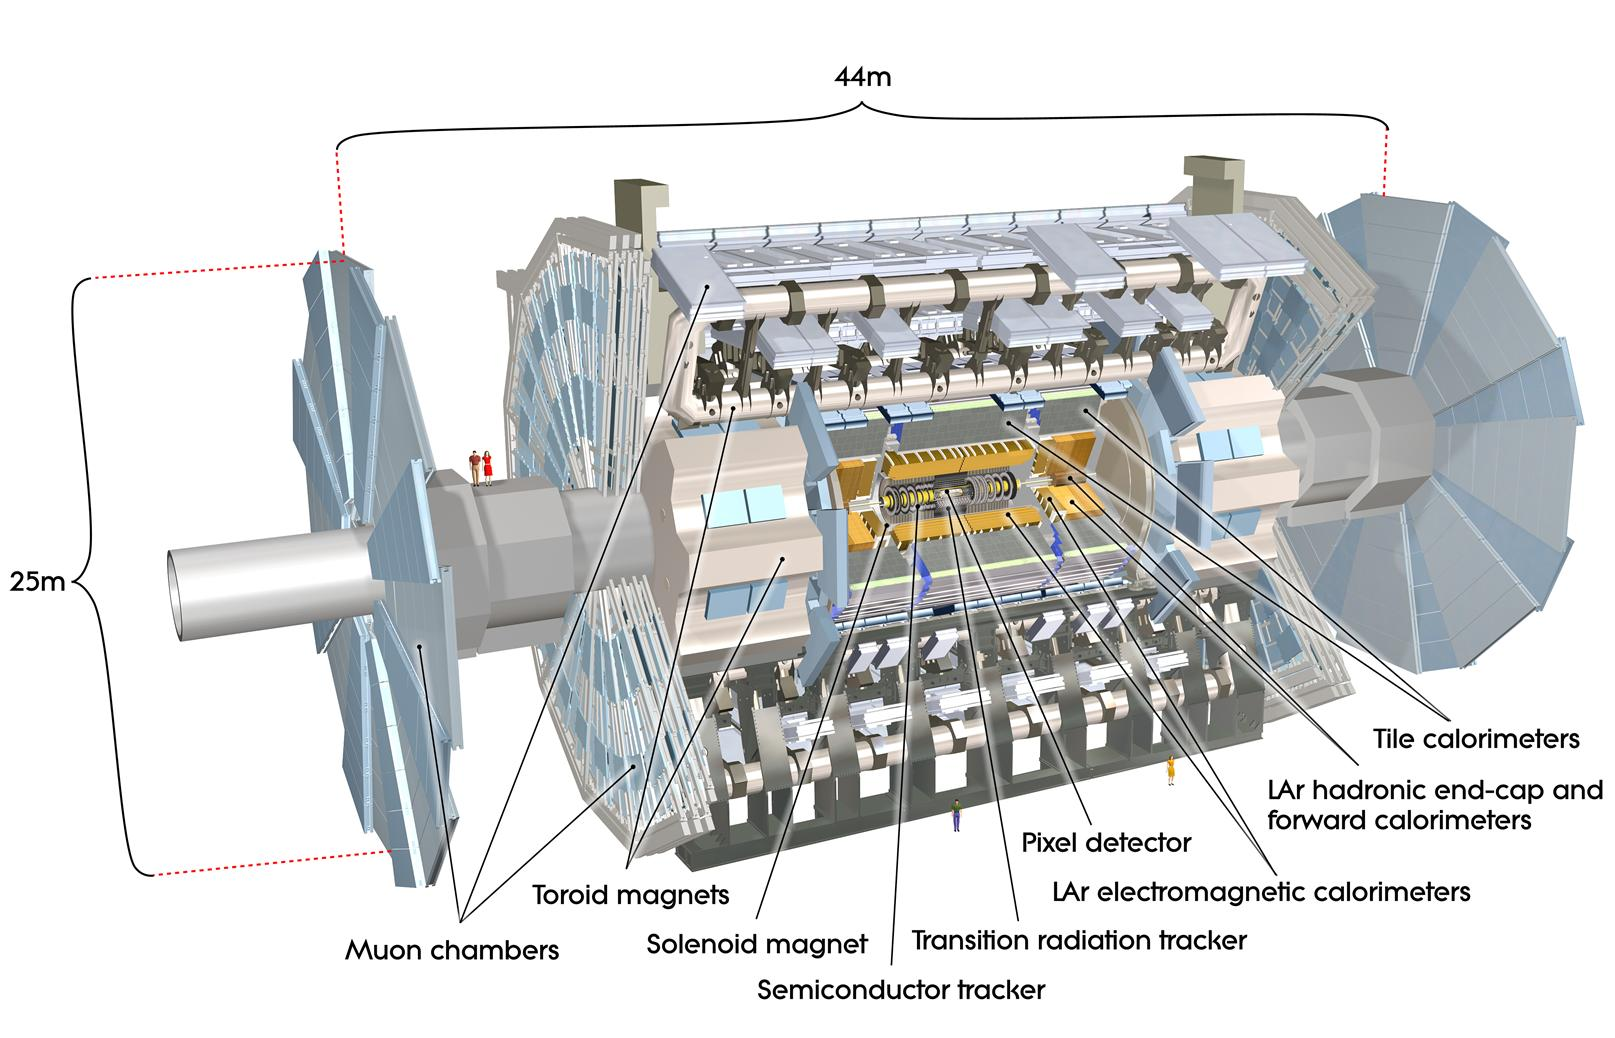
\includegraphics[width=0.8\textwidth]{figures/atlas.png}
    \centering
    \caption{The ATLAS detector showing various sub-detector systems.}
    \label{fig:atlas}
\end{figure}

The ATLAS detector is a multi-purpose detector designed to investigate a wide range of physics, including the search for the Higgs boson in Run I and many searches beyond the SM. The detector measures 46 m long, 25 m in diameter, and it has three main layers of sub-detectors to detect particles created from $pp$ collisions at the Interaction Point (IP). Figure~\ref{fig:atlas} shows the ATLAS detector and the sub-detector systems: the Inner detector, the electromagnetic and hadronic calorimeters, and the muon spectrometer. In this section, the coordinate system, the sub-detectors, and the magnet system of the ATLAS detector are described.

\subsection{Coordinate System}
\label{sec:atlas:coordinate}
In the ATLAS coordinate system, the IP is defined as the origin of the coordinate system. The beam line defines the z-axis, and the x-y plane perpendicular to the beam line is referred to as the transverse plane. The positive x-axis points from the IP to the center of the LHC ring, and the positive y-axis is defined as pointing upward. The azimuthal angle $\phi$ is defined as the angle from the x-axis. The polar angle $\theta$ is defined as the angle from the positive z-axis, and it is also expressed as pseudo-rapidity $\eta$,

\begin{equation}
    \label{eq:eta}
    \eta = -\ln (\tan (\frac{\theta}{2})),
\end{equation}
%
which is a particularly useful quantity because of Lorentz invariance under a boost along the z axis. The distance $\Delta R$ is defined in $\eta$-$\phi$ plane as $\Delta R = \sqrt{\Delta \eta^{2} + \Delta \phi^{2}}$.

\subsection{The Inner Detector}
\label{sec:atlas:id}
The Inner Detector (ID) is a particle tracker designed to measure the charge and transverse momentum of charged particles and to reconstruct the primary and secondary vertices. It consists of cylindrical barrels and two end-cap disks from three sub-detectors centered around the IP. The ID covers the pseudo-rapidity region $|\eta| < 2.5$. 

The detector is immersed  in a 2 T magnetic field generated by the superconducting solenoid magnets, and the magnetic field is used to bend trajectories of charged particles. The transverse momentum and the charge of a particles are then determined from the curvature of the trajectory.

The sub-detectors of the ID, the Pixel tracker, the semiconductor tracker (SCT), and the transition radiation tracker (TRT), are discussed in the following sections.

\subsubsection{Pixel Detector}
\label{sec:atlas:pixel}

The Pixel detector is a semiconductor detector in the innermost part of the ATLAS tracking system. The detector consists of 4 concentric layers of barrel detectors and 3 disk detectors at each end-cap region. The barrels and disks are made of a rectangular Pixel modules containing 80.4 millions pixels of the size 50$\times$400 \si{\micro\meter^{2}} (6 millions pixels of the size 50$\times$250 \si{\micro\meter^{2}} for the IBL)~\cite{1748-0221-10-06-C06012}. As a charged particle traverse through pixels, the currents generated by ionizing electrons are measured and registered as hits. The pixels provide spatial information with resolution of $\sim$ 8 \si{\micro\meter} in radial direction and $\sim$ 75 \si{\micro\meter} in the beam axis, and the information is used for momentum measurements as well as reconstruction of primary and secondary vertices. In Run 2, the Insertable B-Layer (IBL)~\cite{Abbott:2307576} was installed to maintain and improve the performance of the ATLAS detector under increasing pile-up.

\subsubsection{Semi-conductor Tracker}
\label{sec:atlas:sct}

The SCT is the next tracking system following the Pixel detector. Similar to the Pixel detector, the SCT consists of 4 layers of barrel detectors and 9 disk detectors at each end-cap region~\cite{Abdesselam:974073,Abdesselam:973395}. Each barrel/disk is made of SCT modules containing double-sided silicon strips, measuring 80 \si{\micro\meter} wide and 12 \si{\centi\meter} long\footnote{There are two versions of SCT strips in end-cap modules with lengths of 7 and 12 \si{cm}.}. Strips are positioned parallel (perpendicular) to the beam axis in the barrel (end-cap) region. Because a single strip can only provide spatial information in ($r$-$\phi$) direction in barrel and ($z$-$\phi$) direction in end-cap region, double-sided strips are displaced by a relative angle of 40 \si{\milli\radian} to provide three-dimensional spatial measurements of charged particles. The SCT has a spatial resolution of 17 \si{\micro\meter} in radial direction and 580 \si{\micro\meter} in $z$ direction. The information collected by the SCT is used for charge and transverse momentum measurements and reconstruction of vertices.


\subsubsection{Transition Radiation Tracker}
\label{sec:atlas:trt}

The TRT is the outermost tracking system in the ID, covering the region $|\eta| < $ 2.0. The barrel region is covered by 52,544 straw tubes aligned parallel to the beam axis. The end-cap region is covered by 122,800 straw tubes aligned in radial direction. Each straw tube is filled with a Xe-based gas mixture, and a wire is placed at the center of the tube, acting as an anode. When a charged particle traverses the detector, it ionizes the gas mixture inside straws, producing a cascade of electrons. These electrons from the ionization drift toward the center wire, creating signal for the readout electronics with the intrinsic resolution of a single straw tube of $\sim$120~\si{\micro\meter}~\cite{Vogel:1537991}. 

The TRT also provides important information on particle identification. The spaces between straws are filled with polymer fiber (barrels) and foils (end-caps) for the production of transition radiation. When a highly relativistic charged particle passes through them, photons may be emitted by transition radiation, and these photons can be absorbed by the gas mixture, resulting in higher readout signals than usual, called high-threshold hits. The effect is stronger for electrons due to larger relativistic factor ($\gamma = E/m$) than particles with a lower boost such as hadrons. Therefore, the high-threshold hits in the TRT can be used for electron/pion identification~\cite{ATLAS-CONF-2011-128}.

\subsection{The Calorimeters}
\label{sec:atlas:calorimeter}

\begin{figure}[!htb]
    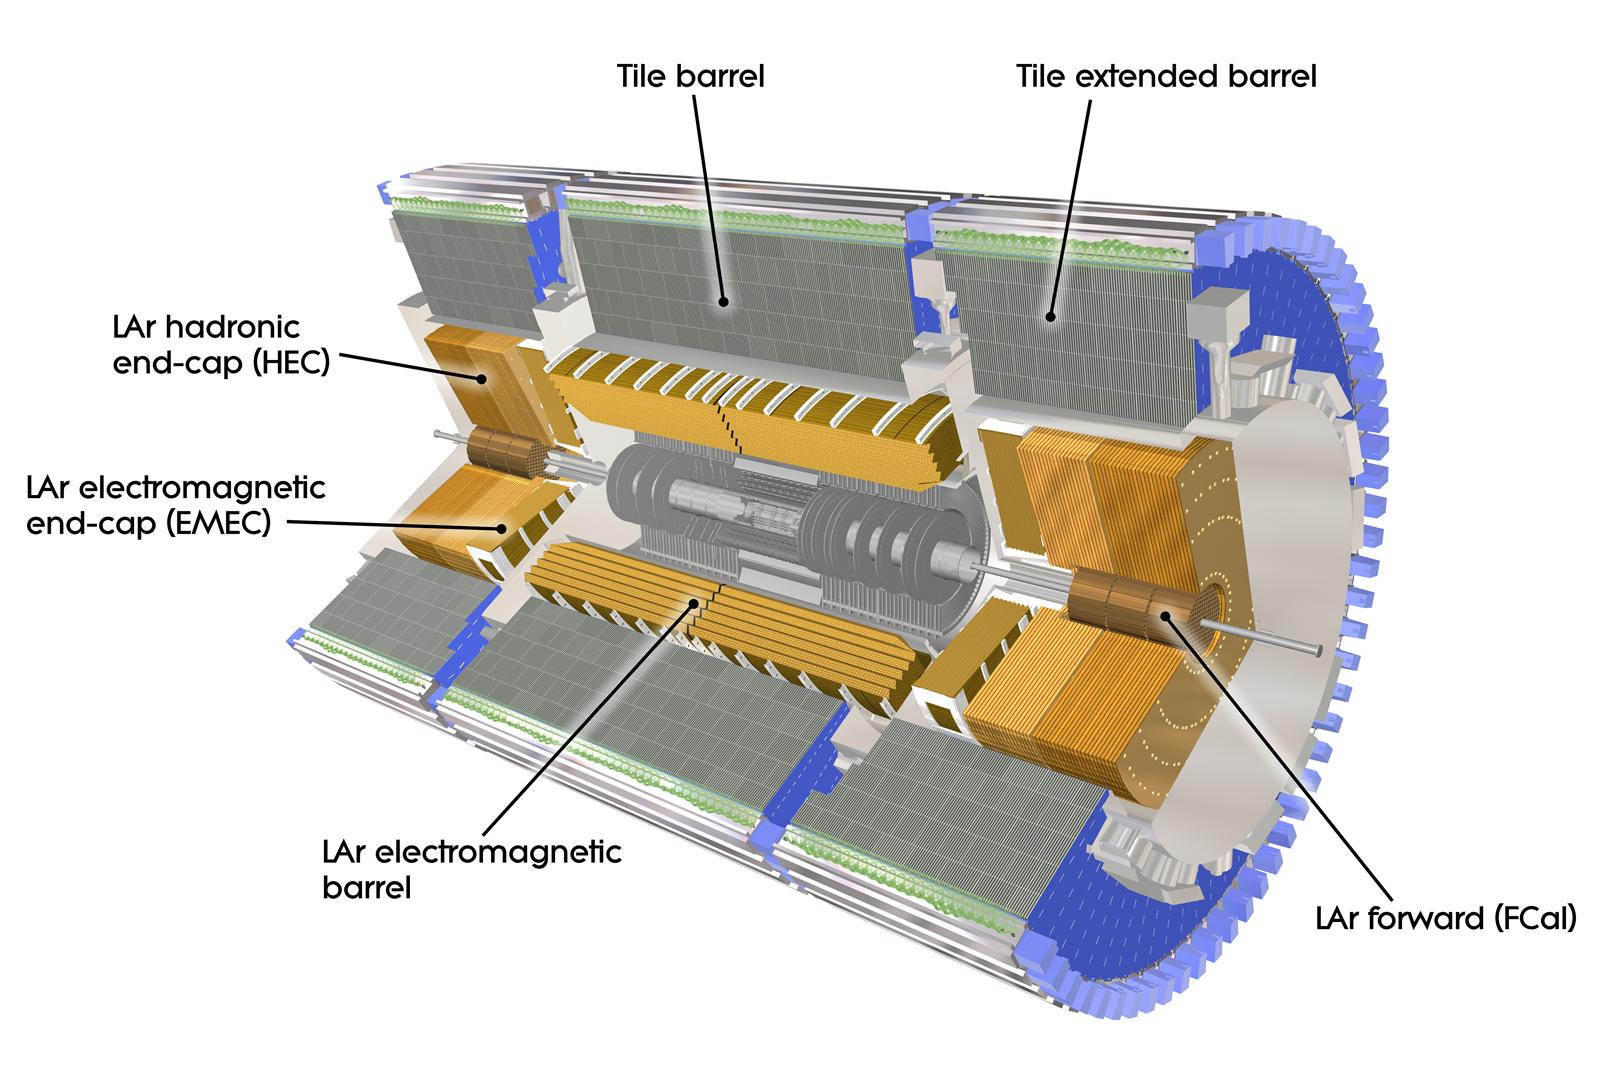
\includegraphics[width=0.8\textwidth]{figures/calorimeter.jpg}
    \centering
    \caption{The ATLAS calorimeter system.}
    \label{fig:calorimeter}
\end{figure}


The ATLAS calorimetry system, shown in Figure~\ref{fig:calorimeter}, consists of two sub-systems, the Liquid Argon (LAr) calorimeters~\cite{1742-6596-293-1-012044} and the tile calorimeters (TileCals)~\cite{HenriquesCorreia:2004868}. The calorimeters are designed to measure the energy deposited by a particle as it traverses through the detector, and the signals from calorimeters are also used for the trigger system. Based on its usage, the calorimeters can be grouped into two sets of calorimeters: the Electromagnetic (EM) calorimeters and hadronic calorimeters.


\subsubsection{Electromagnetic Calorimeter}
\label{sec:atlas:EMcal}
The EM calorimeters (EMC) are located outside the ID and the solenoid magnet, and they are designed to measure the energy deposition from electrons and photons. They are composed of two LAr calorimeters, the EM End-Cap calorimeter (EMEC) covering the region of $|\eta|<$ 1.475 and the EM Barrel (EMB) calorimeter covering the region of 1.375 $<|\eta|<$ 3.2. The LAr calorimeters are composed of layers of high density material (Pb) and LAr sampling layer interspaced for absorption of electron/photons and energy measurement, respectively. The first layer of the LAr calorimeters is called \textit{presampler} which is a thin layer of liquid argon without absorber in front, and it is used to correct for the energy loss before a particle reach the calorimeter. The LAr calorimeters are called sampling calorimeters because only a small fraction of the deposited energy is measured by sampling layers.

When an electron or a photon enters the calorimeters, the electron/photon interacts with the absorber layers, creating the initial EM shower via bremsstrahlung and pair-production. The EM shower is amplified and collected by the sampling layers. The EM calorimeters have the minimum number of radiation length of 24 $X_{0}$~\cite{ATLAS-LAR-CALORIMETER}.




\subsubsection{Hadronic Calorimeter}
\label{sec:atlas:Hcal}
Hadrons are less likely to produce bremsstrahlung radiation due to heavier mass, and they can traverse through the EMC without losing significant energy. Therefore, the hadronic calorimeters are located outside the EMC to measure the energy of hadrons penetrating the EMC. The hadron calorimeters are composed of both LAr calorimeters and TileCals.

The hadronic LAr calorimeters consists of two parts, the hadronic end-cap calorimeter (HEC) covering the region of 1.5 $<|\eta|<$ 3.2 and the forward calorimeter (FCAL) covering the region of 3.1 $<|\eta|<$ 4.9. The principal of hadronic LAr calorimeters is the same as EM LAr calorimeters. The HEC is divided into four longitudinal layers with copper absorber. The FCAL consists of one EM layer with copper as absorber and two hadronic layers with tungsten as passive material. When a hadron enters the hadronic LAr calorimeters, the particle interacts with nuclei of the absorber material via strong force, creating a hadronic shower. The hadronic shower is sampled by sampling layers.

 TileCals are designed to cover the central barrel region ($|\eta| <$ 1.0) and the extended barrel region (0.8 $<|\eta|$ 1.7). The TileCals are made of alternating layers of iron and scintillating tiles. Hadrons entering the absorber layers produce hadronic showers, and the secondary particles from the showers interact with the scintillating tiles to produce lights. The photons are delivered to photomultipliers via wave-length shifting fibers and registered as calorimeter cluster hit.

The TileCals, combined with the hadronic LAr calorimeters, provide measurement of hadrons, jets, taus, and missing transverse energy ($E_{T}^{miss}$).


\subsection{The Muon Spectrometer}
\label{sec:atlas:ms}

\begin{figure}[!htb]
    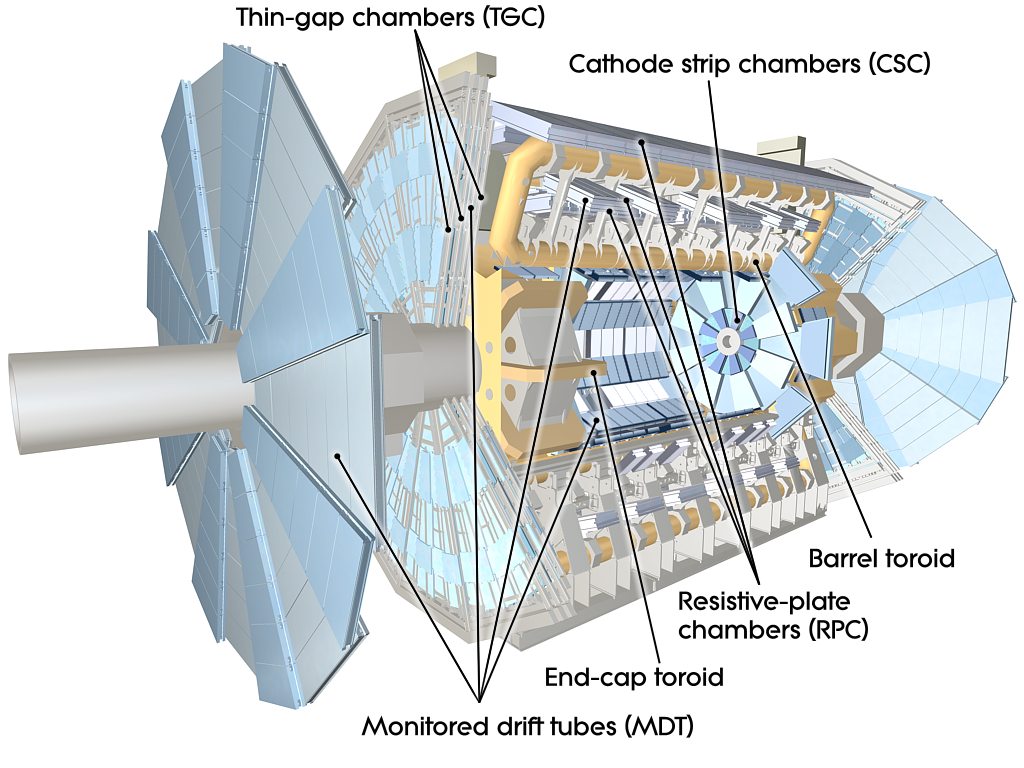
\includegraphics[width=0.7\textwidth]{figures/ms.png}
    \centering
    \caption{The ATLAS Muon Spectrometer}
    \label{fig:ms}
\end{figure}
The Muon Spectrometer (MS) is the outermost detector in the ATLAS detector, responsible for muon identification, momentum measurements, and muon trigger information. The MS is designed to provide high $p_{T}$ momentum measurement with resolution of $\sigma_{p_{T}} / p_{T} = 10\%$, independent from the ID. The MS consists of four sub-detector systems. The Resistive Plate Chambers (RPCs) and the Thin Gap Chambers (TGCs) are used for muon triggering. The Monitored Drift Tubes (MDTs) and the Cathode Strip Chambers (CSCs) allow precise tracking and momentum measurements. The MS barrel region covers the region of $|\eta|<$ 1, and the coverage is extended to $|\eta|<$ 2.7 in the end-cap. Magnetic field of 0.5 T~\cite{ARNAUD2008265} is provided by a system of a large toroidal magnet (barrel) and two smaller toroidal magnets (end-cap). A layout of the MS is shown in Figure~\ref{fig:ms}.

\subsubsection{Monitored Drift Tube Chambers}
\label{sec:atlas:mdt}

The MDT chambers provide precision momentum measurements using chambers of drift tubes filled with a gas mixture of Ar (97\%) and $\mathrm{CO}_{2}$(3\%). The barrel MDT chambers are arranged in three layers, covering the region of $|\eta|<$ 1.1. The end-cap MDT chambers are arranged in three wheels, covering the region of 1.1 $<|\eta|<$ 2.7. Each chamber has 6-8 layers of drift tubes of 3 \si{\centi\meter} in a diameter, and a tungsten-rhenium wire is placed at the center as an anode. The principal of particle detection is similar to the TRT, but the drift tubes are arranged perpendicular to the beam axis in the barrel layers and tangential in the end-cap layers. This configuration allows the MDT to measure the curvature of a muon in $\eta$-$z$ plane under the toroidal magnetic field.

\subsubsection{Cathode Strip Chambers}
\label{sec:atlas:csc}

The CSCs are located on the innermost wheel of the end-caps, covering the region of 2.0 $<|\eta|<$ 2.7. In this region, the MDTs would not operate properly due to the high rates of muons at this region. Instead, sixteen CSCs on each end-cap provide precise tracking for high density muons with the resolution of 60 \si{\micro\meter} in $\eta$-$z$ plane and 5 \si{\milli\meter} in the radial direction. The CSCs are multi-wire proportional chambers with segmented cathode strips in alternating alignment. The multi-wires are aligned in the radial direction, and the strips are aligned perpendicular or parallel to the wires to provide 2 dimensional measurements in both $\eta$ and $\phi$ directions.


\subsubsection{Resistive Plate Chambers}
\label{sec:atlas:rpc}

The RPCs provide trigger capability for the muon trigger and measurements in $\eta$, $\phi$ coordinates in the barrel region. There are three RPCs arranged in concentric cylindrical shells around the beam axis. The two inner RPCs are placed at the radii of 5 and 7.5 \si{\meter} to provide the low-$p_{T}$ trigger information. The outer RPCs are installed at the radius of 10 \si{\meter} to provide high-$p_{T}$ trigger information. Each chamber consists of two parallel resistive plates separated by a 2 \si{\milli\meter} gap filled with a gas mixture based on $\mathrm{C}_{2}\mathrm{H}_{2}\mathrm{F}_{4}$. A muon track passing through the RPCs ionizes the gas, and the signal is multiplied and read out by each chamber, providing 6 measurements for each track.

\subsubsection{Thin Gap Chambers}
\label{sec:atlas:tgc}

The TGCs are designed to provide trigger information and $\phi$ measurements (non-bending direction) in the end-cap region. Similar to the CSCs, the TGCs are made of multi-wire proportional chambers filled with a gas mixture of 55\% $\mathrm{CO}_{2}$ and 45\% $\mathrm{C}_{5}\mathrm{H}_{12}$. The strips are oriented in radial direction, allowing measurements in $\phi$. The TCGs consists of 4 layers of chambers on each end-cap, covering the region of 1 $<|\eta|<$ 2.7.


\subsection{The ATLAS Magnet}
\label{sec:atlas:magnet}

The ATLAS detector has three major superconducting magnet systems surrounding the ID and the MS: the Central Solenoid magnet and the Barrel/End-cap Toroid magnets.

\subsubsection{Central Solenoid Magnet}
\label{sec:atlas:solenoid}
The Central Solenoid magnet surrounds the ID, producing a 2 T magnetic field. The solenoid is designed to bend the trajectory of a charged particle in $r$-$\phi$ plane. The curvatures of charged particles are used for the measurements of charge-to-momentum ratio. The solenoid magnet measures 2.4 \si{\meter} in diameter and 5.3 \si{\meter} in length, and 7.73 \si{\kilo\ampere} of current is applied to generate the solenoidal magnetic field.


\subsubsection{Toroid Magnets}
\label{sec:atlas:toroid}

In the outer region of the ATLAS detector, two superconducting toroid magnet systems are used to generate a magnetic field within the MS. The barrel toroid are composed of 8 separate coils made of Al/NbTi/Cu conductor with 120 turns. The toroid measures 20.1 \si{\meter} in diameter and 25.3 \si{\meter} in length. The end-cap toroid has 8 coils with 116 turns, and the coils are made of the same material as the barrel toroid. The nominal current of 20.5 \si{\kilo\ampere} is applied to generate a magnetic field of 1-2 T with the field integral of 2 to 8 Tm.

\section{The ATLAS Trigger System}
\label{sec:atlas:daq}

\begin{figure}[!htb]
    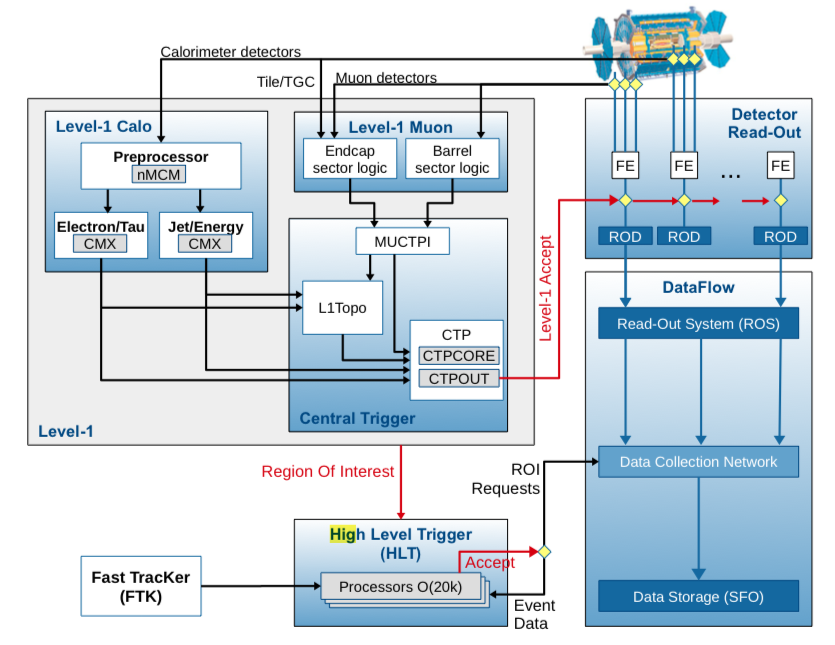
\includegraphics[width=0.8\textwidth]{figures/tdaq.png}
    \centering
    \caption{Layout of the ATLAS Trigger and data acquisition system in Run 2.}
    \label{fig:tdaq}
\end{figure}

The ATLAS trigger system is designed to select interesting events from raw event data at high rate, generated by $pp$ collisions. In Run 2, the LHC collide proton bunches every 25 \si{\nano\second}, resulting in about a billion $pp$ collisions per second at $\langle\mu\rangle = 24.9$ (in 2016). Due to the limited bandwidth and computing resources, it is impossible to record all events from the collisions. Therefore, the ATLAS trigger system is implemented to reduce the data taking rate from 40 \si{\mega\hertz} to 100 \si{\kilo\hertz}. In Run 2,several upgrades have been performed in both hardware and software to maintain data quality in the environment with increasing pile-up, higher instantaneous luminosity at the center-of-mass energy of $\sqrt{s}=$13 TeV.

The trigger system in Run 2 consists of a hardware-based Layer 1 (L1) trigger and a software-based High Level Trigger (HLT). Figure~\ref{fig:tdaq} shows the ATLAS trigger and data acquisition system in Run 2. The events accepted by the trigger system are further processed by the Data Acquisition (DAQ) system where the information from front-end electronics of each detector component are used to build an individual event. The reconstructed events from DAQ are sent to Data Storage (SFO) for permanent storage.



\subsection{Level 1 Trigger}
\label{sec:atlas:l1trigger}

The L1 trigger is a hardware-based trigger system that operates at the maximum rate of 100 \si{\kilo\hertz}~\cite{1742-6596-762-1-012003}. The main components of the L1 trigger consist of the L1 calorimeter trigger system and the L1 muon trigger system . The L1 trigger uses custom electronics to make fast decisions and find regions of interest (RoI) in the detector where potentially interesting activities are registered in the calorimeters or the MS.

A list of trigger selection is developed based on the physics goal of the collaboration and the needs of individual analyses. The list is called the Trigger Menu~\cite{VazquezSchroeder:2287548}. The L1 trigger accepts the events with high $p_{T}$ tracks, jets, or large $E_{T}^{miss}$ that satisfies one of the trigger menu. The events accepted by the L1 trigger is passed to the software-based trigger system.


\subsection{High Level Trigger}
\label{sec:atlas:hlt}

The HLT makes the decision on events based on full information from the detector read-out in the RoI passed by the L1 trigger. This includes a fast reconstruction of the ID tracks. The HLT has the average output rate of 1 \si{\kilo\hertz}~\cite{1742-6596-762-1-012003}, constrained by data storage limitation. 


